\documentclass[aspectratio=169]{beamer}
\usepackage{hyperref}
\usepackage{xcolor}
\usepackage{graphicx}
\usepackage{tikz}
\usetikzlibrary{positioning}
\usepackage{authoraftertitle}
\usepackage{fontspec}

\setsansfont{Oswald}[Path=./OswaldFontFiles/,Scale=0.9,Extension=.ttf,UprightFont=*-Regular,BoldFont=*-Bold]
    
\setromanfont{Lato}[Path=./LatoFontFiles/,Scale=0.9,Extension=.ttf,UprightFont=*-Regular,BoldFont=*-Bold]    

\setbeamertemplate{navigation symbols}{}
\setbeamertemplate{background}{\tikz[overlay, remember picture]%
  \node[anchor=south] at (current page.south)
     {
\includegraphics[width=.45\paperwidth]{img/slider-in}};}

\author{Lect. Dr. \c{S}otropa Diana}
\title{Prezentare}
\newcommand\Facultate{Facultatea de Matematic\u{a} \c{s}i Informatic\u{a}}
\newcommand\Universitate{Universitatea Babe\c{s}-Bolyai}
\newcommand\Adresa{Str. Mihail Kog\u{a}lniceanu nr. 1\\ Cluj-Napoca, Cluj, Rom\^{a}nia}
\newcommand\Website{www.cs.ubbcluj.ro}
\newcommand\DataPrezentarii{24 Noiembrie 2021}

\usepackage{CSTheme_RO}

\begin{document}

%GENERARE PAGINA DE TITLU
%custom/title.tex
% Title slide frame
\begin{frame}[plain]
\begin{tikzpicture}[remember picture,overlay]
% Background image
\node[above right,inner sep=0pt] at (current page.south west)
{
    \includegraphics[width=\paperwidth]{img/blueCS_background.png}
};
    
% Title
\node[anchor=center, color=yellowCS, align=center, text width=14cm] (title) at ([yshift=0.5cm]current page.center)
{
    \Huge \MyTitle
};

% Separator Line
\draw[yellowCS, ultra thick] ([yshift=-0.5cm, xshift=-4cm]title.south) -- ([yshift=-0.5cm, xshift=4cm]title.south);

% Author 
\node[anchor=north, color=white, align=center] (author) at ([yshift=-1cm]title.south)
{
    \Large \MyAuthor
};

% Facultate
\node[anchor=north, color=yellowCS, align=center] (date1) at ([yshift=-0.8cm]author.south)
{
    \large \Facultate
};

% Universitate
\node[anchor=north, color=white, align=center] (date2) at ([yshift=-0.1cm]date1.south)
{
    \large \Universitate
};

% Logo CS
\node[anchor=north west] at ([xshift=1cm, yshift=-1cm]current page.north west)
{
    
\includegraphics[width=2cm]{img/CS_white_logo.png}
};

% Logo UBB
\node[anchor=north east] at ([xshift=-1cm, yshift=-1cm]current page.north east)
{
    
\includegraphics[width=2cm]{img/Sigla_UBB_claudiopolitana_alb.png}
};

\end{tikzpicture}
\end{frame}


%GENERARE PAGINA DE SECTIUNE CARE CONTINE TREI TEXTE SALVATE IN \sectionTitle, \sectionSubtitle, \sectionMotto
%SECTION TEMPLATE 1
%custom/section-template-1.tex
\newcommand\sectionTitle{\Facultate}
\newcommand\sectionSubtitle{\Universitate}
\newcommand\sectionMotto{Motto: Your Career, Our Duty}
% Section 1 slide frame
\begin{frame}[plain]
\begin{tikzpicture}[remember picture,overlay]
% Background image
\node[above right,inner sep=0pt] at (current page.south west)
{
    \includegraphics[width=\paperwidth]{img/blueCS_background.png}
};

% Center logos around the middle
% Left logo at x=6cm, right logo at x=10cm would be symmetric (X=8 is center).
\node[anchor=center] at ([yshift=1.5cm, xshift=-2cm]current page.center)
{
    
\includegraphics[width=1.85cm]{img/facultatea de matematica_alba_transp.png}
};

\node[anchor=center] at ([yshift=1.5cm, xshift=2cm]current page.center)
{
    
\includegraphics[width=2cm]{img/CS_white_logo.png}
};

% Separator Line
\draw[yellowCS, ultra thick] ([yshift=0cm, xshift=-4cm]current page.center) -- ([yshift=0cm, xshift=4cm]current page.center);
  
% section title
\node[anchor=north, color=white, align=center, text width=14cm] at ([yshift=-1cm]current page.center) {\huge \sectionTitle};
\node[anchor=north, color=white, align=center, text width=14cm] at ([yshift=-2.5cm]current page.center) {\Large \sectionSubtitle};


\end{tikzpicture}
\end{frame}


%CONTINUT EFECTIV SLIDE-URI
\begin{frame}{Despre noi}
\begin{itemize}
    \item Component\u{a} important\u{a} a unei Universit\u{a}\c{t}i de mare prestigiu \c{s}i anvergur\u{a}, Facultatea de Matematic\u{a} \c{s}i Informatic\u{a}, este \^{i}n acest moment o \^{i}mpletire fericit\u{a} de tradi\c{t}ie \c{s}i actualitate, de modernitate \c{s}i experien\c{t}\u{a}.
    \item Clasificarea domeniului Matematic\u{a} din topurile Best Global Universities și The world’s best universities for Mathematics este o recunoa\c{s}tere fireasc\u{a} a valorii \c{s}colii de Matematic\u{a} din Rom\^{a}nia \c{s}i \^{i}n particular de la Universitatea Babe\c{s}-Bolyai din Cluj-Napoca, valoare bazat\u{a} pe tradi\c{t}ie, munc\u{a} \c{s}i seriozitate \^{i}ntr-un climat de competi\c{t}ie onest\u{a}.
\end{itemize}
\end{frame}

%CONTINUT EFECTIV SLIDE-URI
\begin{frame}{Despre noi}
 \begin{minipage}{0.55\linewidth}
        \begin{itemize}
            \item Dac\u{a} Cluj-Napoca a devenit un centru important de IT\&C pe harta Europei, acest lucru s-a ȋnt\^{a}mplat \c{s}i datorit\u{a} bunei preg\u{a}tiri a absolven\c{t}ilor de Informatic\u{a} din facultatea noastr\u{a}. 
            \item Absolven\c{t}ii de Informatic\u{a} din Universitatea Babe\c{s}-Bolyai sunt extrem de bine aprecia\c{t}i de c\u{a}tre companiile de profil, exist\^{a}nd o adev\u{a}rat\u{a} „v\^{a}n\u{a}toare de creiere” ȋnc\u{a} din anii facult\u{a}\c{t}ii.
        \end{itemize}
 \end{minipage}
 \begin{minipage}{0.4\linewidth}
    \begin{figure}[h]
        \centering
        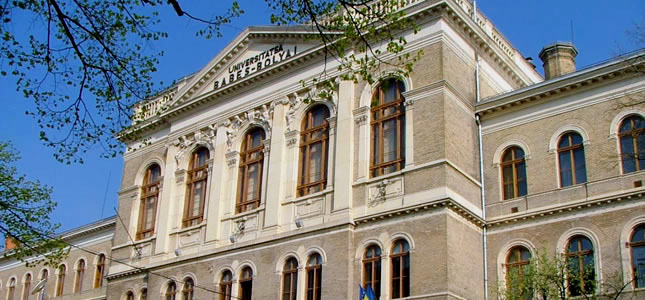
\includegraphics[height=0.2\textheight]{img/uploads/1.jpg}
    \end{figure}
    \begin{figure}[h]
        \centering
        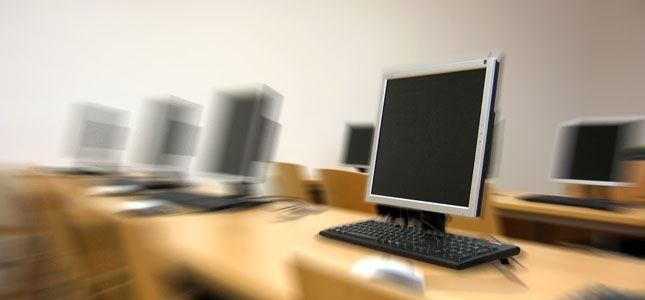
\includegraphics[height=0.2\textheight]{img/uploads/4.jpg}
    \end{figure}
    \begin{figure}[h]
        \centering
        
\includegraphics[height=0.2\textheight]{img/uploads/7.jpg}
    \end{figure}
\end{minipage}
\end{frame}

%GENERARE PAGINA DE SECTIUNE CARE CONTINE DOUA TEXTE SALVATE IN \sectionTitle, \sectionSubtitle
%SECTION TEMPLATE 2
%custom/section-template-2.tex
\renewcommand*\sectionTitle{Departamente}
\renewcommand*\sectionSubtitle{\Facultate}
\include{custom/section-template-2}

%CONTINUT EFECTIV SLIDE-URI
\begin{frame}{Departamente}
\begin{itemize}
    \item Departamentul de Matematic\u{a}
    \item Departamentul de Informatic\u{a}
    \item Departamentul de Matematic\u{a} și informatic\u{a} al liniei maghiare
\end{itemize}
\end{frame}

%GENERARE PAGINA DE SECTIUNE CARE CONTINE DOUA TEXTE SALVATE IN \sectionTitle, \sectionSubtitle
%SECTION TEMPLATE 2
%custom/section-template-2.tex
\renewcommand*\sectionTitle{Specializ\u{a}ri}
\renewcommand*\sectionSubtitle{\Facultate}
\include{custom/section-template-2}

%CONTINUT EFECTIV SLIDE-URI
\begin{frame}{Specializ\u{a}ri nivel licen\c{t}\u{a}}
\begin{minipage}[t]{0.48\linewidth}
\begin{block}{\centering Domeniul Matematic\u{a}}
        \begin{itemize}
            \item Matematic\u{a} rom\^{a}n\u{a}
            \item Matematic\u{a} maghiar\u{a}
            \item Matematic\u{a} informatic\u{a} rom\^{a}n\u{a}
            \item Matematic\u{a} informatic\u{a} maghiar\u{a}
            \item Matematic\u{a} informatic\u{a} englez\u{a}
        \end{itemize}
\end{block}        
 \end{minipage}
  \hspace{0.08\textwidth}%
 \begin{minipage}[t]{0.42\linewidth}
\begin{block}{\centering Domeniul Informatic\u{a}}        
        \begin{itemize}
            \item Informatic\u{a} rom\^{a}n\u{a}
            \item Informatic\u{a} englez\u{a}
            \item Informatic\u{a} maghiar\u{a}
            \item Informatic\u{a} german\u{a}
        \end{itemize}
 
 \end{block}        
\end{minipage}
\end{frame}


%CONTINUT EFECTIV SLIDE-URI
\begin{frame}{Specializ\u{a}ri nivel master}
\begin{minipage}[t]{0.5\linewidth}
\begin{block}{\centering Informatic\u{a}}
        {\tiny $\bullet$ Analiza datelor \c{s}i modelare maghiar\u{a}
            \newline $\bullet$ Baze de date rom\^{a}n\u{a}
            \newline $\bullet$ Calcul de \^{i}nalt\u{a} performan\c{t}\u{a} \c{s}i analiza volumelor mari de date englez\u{a}
            \newline $\bullet$ Metode moderne \^{i}n predarea informaticii rom\^{a}n\u{a}
            \newline $\bullet$ Metode moderne \^{i}n predarea informaticii maghiar\u{a}
            \newline $\bullet$ Inginerie software englez\u{a}
            \newline $\bullet$ Inteligen\c{t}\u{a} computa\c{t}ional\u{a} aplicat\u{a} englez\u{a}
            \newline $\bullet$ Programare bazat\u{a} pe componente englez\u{a}
            \newline $\bullet$ Proiectarea \c{s}i dezvoltarea aplica\c{t}iilor Enterprise maghiar\u{a}
            \newline $\bullet$ Sisteme distribuite \^{i}n internet rom\^{a}n\u{a}
            \newline $\bullet$ Sisteme informatice avansate: modelare, proiectare, dezvoltare german\u{a}, englez\u{a}
}
\end{block}        
 \end{minipage}
  \hspace{0.04\textwidth}%
 \begin{minipage}[t]{0.4\linewidth}
\begin{block}{\centering Matematic\u{a}}        
        {\tiny
            $\bullet$ Matematic\u{a} computa\c{t}ional\u{a} maghiar\u{a}
            \newline $\bullet$ Metode moderne \^{i}n predarea matematicii rom\^{a}n\u{a}
            \newline $\bullet$ Metode moderne \^{i}n predarea matematicii maghiar\u{a}
            \newline $\bullet$ Matematici avansate englez\u{a}
 }
 \end{block}        
\begin{block}{\centering \c{S}tiin\c{t}e ale Educa\c{t}iei}        
        {\tiny
            $\bullet$ Masterat didactic \^{i}n Informatic\u{a} rom\^{a}n\u{a}
            \newline $\bullet$ Masterat didactic \^{i}n Matematic\u{a} maghiar\u{a}
            \newline $\bullet$ Masterat didactic \^{i}n Informatic\u{a} maghiar\u{a}
            }
 
 \end{block}        
\end{minipage}
\end{frame}
%GENERARE PAGINA DE SECTIUNE CARE CONTINE DOUA TEXTE SALVATE IN \sectionTitle, \sectionSubtitle
%SECTION TEMPLATE 2
%custom/section-template-2.tex
\renewcommand*\sectionTitle{Centre de Cercetare}
\renewcommand*\sectionSubtitle{\Facultate}
\include{custom/section-template-2}

%CONTINUT EFECTIV SLIDE-URI
\begin{frame}{Centre de cercetare\\ acreditate la nivelul Universităţii Babeş-Bolyai}
\begin{itemize}
    \item Centrul de Cercetare Analiză Aplicată, Coordonator: Prof. dr. Radu Precup
    \item Centrul de Cercetare Algebre, Grupuri şi Aplicaţii, Coordonator: Prof. dr. Andrei Mărcuş
    \item Centrul de Cercetare Inteligenţă Computaţională Aplicată, Coordonator: Prof. dr. Horia F. Pop
    \item Centrul de Cercetare Inginerie Software, Coordonator: Conf. dr. Simona Motogna
    \item Centrul pentru Studiul Complexităţii, Coordonator: Conf. dr. Rodica Lung


\end{itemize}
\end{frame}


%CONTINUT EFECTIV SLIDE-URI
\begin{frame}{Grupuri de cercetare pe domeniul Matematică\\ acreditate la nivelul facultăţii}
\begin{itemize}
    \item Grupul de cercetare Analiză şi optimizare, Coordonatori: Prof. dr. Kassay Gábor, Prof. dr. Nicolae Popovici
    \item Grupul de cercetare de Geometrie, Coordonator: Prof. dr. Dorin Andrica
    \item Grupul de cercetare de Analiză complexă, Coordonator: Prof. dr. Gabriela Kohr
    \item Grupul de cercetare Operatori neliniari si ecuaţii diferenţiale, Coordonatori: Prof. dr. Radu Precup, Prof. dr. Adrian Petruşel
    \item Grupul de cercetare Analiză numerică şi stohastică, Coordonator: Prof. dr. Octavian Agratini
    \item Grupul de cercetare de Mecanică si astronomie, Coordonator: Prof. dr. Mirela Kohr
    \item Grupul de cercetare Simulare şi modelare, Coordonator: Conf. dr. Libál András

\end{itemize}
\end{frame}


%CONTINUT EFECTIV SLIDE-URI
\begin{frame}{Grupuri de cercetare pe domeniul Informatică\\ acreditate la nivelul facultăţii}
\begin{itemize}
    \item Grupul de cercetare Învățare automată, Coordonator: Prof. dr. Gabriela Czibula
    \item Grupul de cercetare Sisteme Distribuite şi Comunicaţii Web, Coordonator: Conf. dr. Rareş Boian
    \item Grupul de cercetare Aplicaţii Interdisciplinare Bazate pe Calcul de Inaltă Performanţă, Coordonator: Conf. dr. Virginia Niculescu
    \item Grupul de cercetare Analiza conceptelor formale, Coordonator: Conf. dr. Christian Săcărea
    \item Grupul de cercetare Metaeuristici pentru Sisteme Complexe, Coordonatori: Prof. dr. Anca Andreica, Prof. dr. Laura Dioșan


\end{itemize}
\end{frame}


%GENERARE PAGINA DE CONTACT
%custom/contact.tex
\include{custom/contact}

\end{document}
